% siminos/presentations/GTMAP18/GTMAP18.tex        pdflatex GTMAP18
% $Author: predrag $ $Date: 2018-04-13 12:43:56 -0400 (Fri, 13 Apr 2018) $

%  started with siminos/presentations/GTmath18/GTmath18.tex 2018-02-24
%  started with siminos/presentations/KITP17/UCSB17.tex     2017-01-26
%  started with siminos/presentations/Israel16/Israel16.tex 2016-08-17
%  started with siminos/presentations/GTmap16/GTmap16.tex   2016-08-17
%  started with talks/predrag/NBI16/NBI16.tex               2016-04-25
%  started with talks/predrag/RoySoc16/RoySoc16.tex         2016-04-25

\input ../../inputs/layoutBeamer
\usepackage[font=scriptsize, labelfont=bf]{caption}
\usepackage[
    backend=biber,  %bibtex,
    sorting=nyt,
    %refsection=chapter,
    %citereset=chapter,
    style=numeric, %alphabetic, % %style=authoryear,
    natbib=true,
    style=phys, % aps
    biblabel= brackets, % superscript, %
    articletitle=false, % true,  % false, % aps
    %chaptertitle=true,  % aip;  % false, % aps
    pageranges = true , % aip: the full range
             % = false, % aps: only the first page being printed
    sortlocale=en_US,
    firstinits=true,
    url=false, %true,  %
    doi=false, %true,
    eprint=false
]{biblatex}
\addbibresource{../../bibtex/siminos.bib}
\setbeamerfont{footnote}{size=\tiny}
\input ../../inputs/def % no edits, always from dasbuch/book/inputs
\input ../../inputs/defsBeamer
\renewcommand{\Ssym}[1]{{\ensuremath{m_{#1}}}}    % Boris
% \newcommand{\Ssym}[1]{{\ensuremath{s_{#1}}}}  % ChaosBook

\begin{document}


\title{
{a spatiotemporal theory of}
{\huge turbulence}
    \\
{computational challenges}
}
\author{P. Cvitanovi\'c}
\author[Cvitanovi\'c]
{
  \textcolor{green!50!black}{
  {Predrag~Cvitanovi\'c
  and
  Matt Gudorf
  }	%\inst{1}
  }
}
\institute
{
%  \inst{1}%
GTMAP mini-workshop on dynamics
\\
                Georgia Tech
 }
\date{April 13, 2018}

\begin{frame}
  \titlepage
\end{frame}


\section[what this talk is about]
 {what this talk is about}

\begin{frame}{overview}
\begin{enumerate}
              \item {\Large
what this talk is about
                  }\textcolor{gray}{\small
              \item
turbulence in large domains
              \item
space is time
              \item
bye bye, dynamics
                    }
            \end{enumerate}
\end{frame}

\begin{frame}{do clouds solve PDEs?}

%and do they care what PST hour is it?
%\\
%and at what longitude are they?
%\\
do clouds \textcolor{red}{integrate} Navier-Stokes equations?

\begin{center}
\centerline{\textcolor{red}{\Huge NO!}}
%\end{center}
%for weather prediction, we store sets of weather sequences
%\bigskip\bigskip

%\begin{center}
\begin{minipage}[t]{\textwidth}
	\begin{center}
%\vspace{2ex}
\centerline{
\raisebox{-4.0ex}[5.5ex][4.5ex]
		 {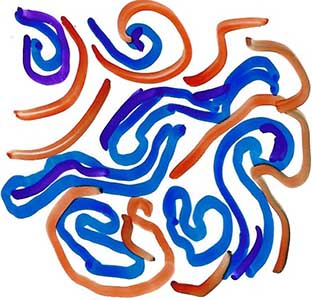
\includegraphics[height=12ex]{Hopf-a}}
~~~ $\Longrightarrow$ ~~ {other swirls} ~~ $\Longrightarrow$ ~~~
	\raisebox{-4.0ex}[5.5ex][4.5ex]
		 {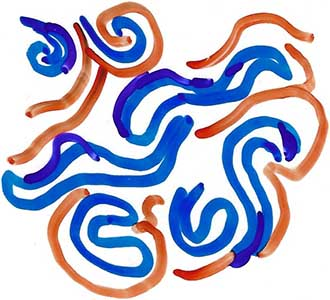
\includegraphics[height=12ex]{Hopf-b}}
          }
	\end{center}
\end{minipage}
\end{center}

do clouds satisfy Navier-Stokes equations?

\bigskip

{\Large yes!}

\centerline{
\textcolor{blue}{they satisfy them \textcolor{red}{\large locally}, everywhere and at all times}
}
\end{frame}

\begin{frame}{part 1}
\begin{enumerate}
              \item {\Large
turbulence in large domains
                  }\textcolor{gray}{\small
              \item
space is time
              \item
spacetime
              \item
bye bye, dynamics
                    }
            \end{enumerate}
\end{frame}


\begin{frame}{goal : enumerate the building blocks of turbulence}
\begin{block}{Navier-Stokes equations} % (1822)}
\[
\dfrac{\partial \bv}{\partial t} + (\bv \cdot \nabla) \bv
	\,=\,
\frac{1}{R} \nabla ^2 \bv
-\nabla p
+ \mathbf{f}
    \,,\qquad
\nabla \cdot \bv = 0,
\]
\end{block}

\hfill{\small
velocity field  $\bv \in \mathbb{R}^3$
;
pressure field $p$
;
driving force $\mathbf{f}$
        }

\medskip

\begin{block}{describe turbulence}
starting from the equations (no statistical assumptions)
\end{block}

\bigskip

% large Reynolds number $R$:
\hfill {\Large\textcolor{red}{}}

\end{frame}

\begin{frame}{challenge : experiments are amazing}
\begin{center}
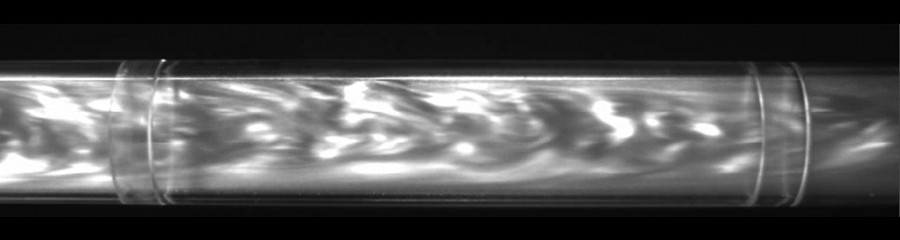
\includegraphics[width=0.7\textwidth]{mullin_puff2200} %pipe}
\end{center}
T. Mullin lab
\begin{center}
\bigskip
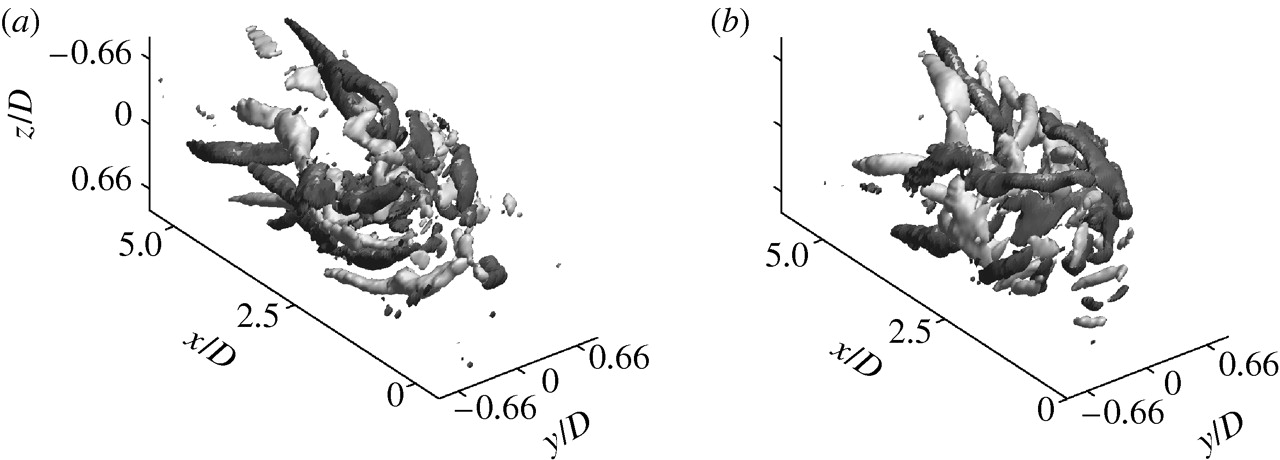
\includegraphics[width=0.7\textwidth]{deLHof09fig6} %pipe}
\end{center}
B. Hof lab
\end{frame}

%\begin{frame}{pipe theory and numerics}
%	\begin{columns}[t]
%	\column{.55\textwidth}
%amazing experiments! \\ amazing numerics! \\ beautiful visualizations !
%
%\bigskip\bigskip
%
%%relative periodic orbits,
%``Exact Coherent Structures'' :
%\\ numerical Navier-Stokes
%
%\medskip
%isosurfaces and cross sections \\ of the streamwise velocity
%
%\medskip
%
%\textcolor{red}{red} (\textcolor{blue}{blue}) streaks
%\\ are \textcolor{red}{faster} (\textcolor{blue}{slower}) \\ than the base flow
%
%\bigskip
%
%{{\tiny Ritter et al., Phys. Rev. Fluids (2018)}}
%
%	\column{.45\textwidth}
%\begin{center}
%  \includegraphics[width=1.0\textwidth,clip=true]
%                    {RZSEA18Fig3}
%\end{center}
%	\end{columns}
%\end{frame}

\section[dynamics in $\infty$ dimensions]
{dynamics in $\infty$ dimensions}

\begin{frame}{can simulate {\Huge large} computational domains}
\begin{center}
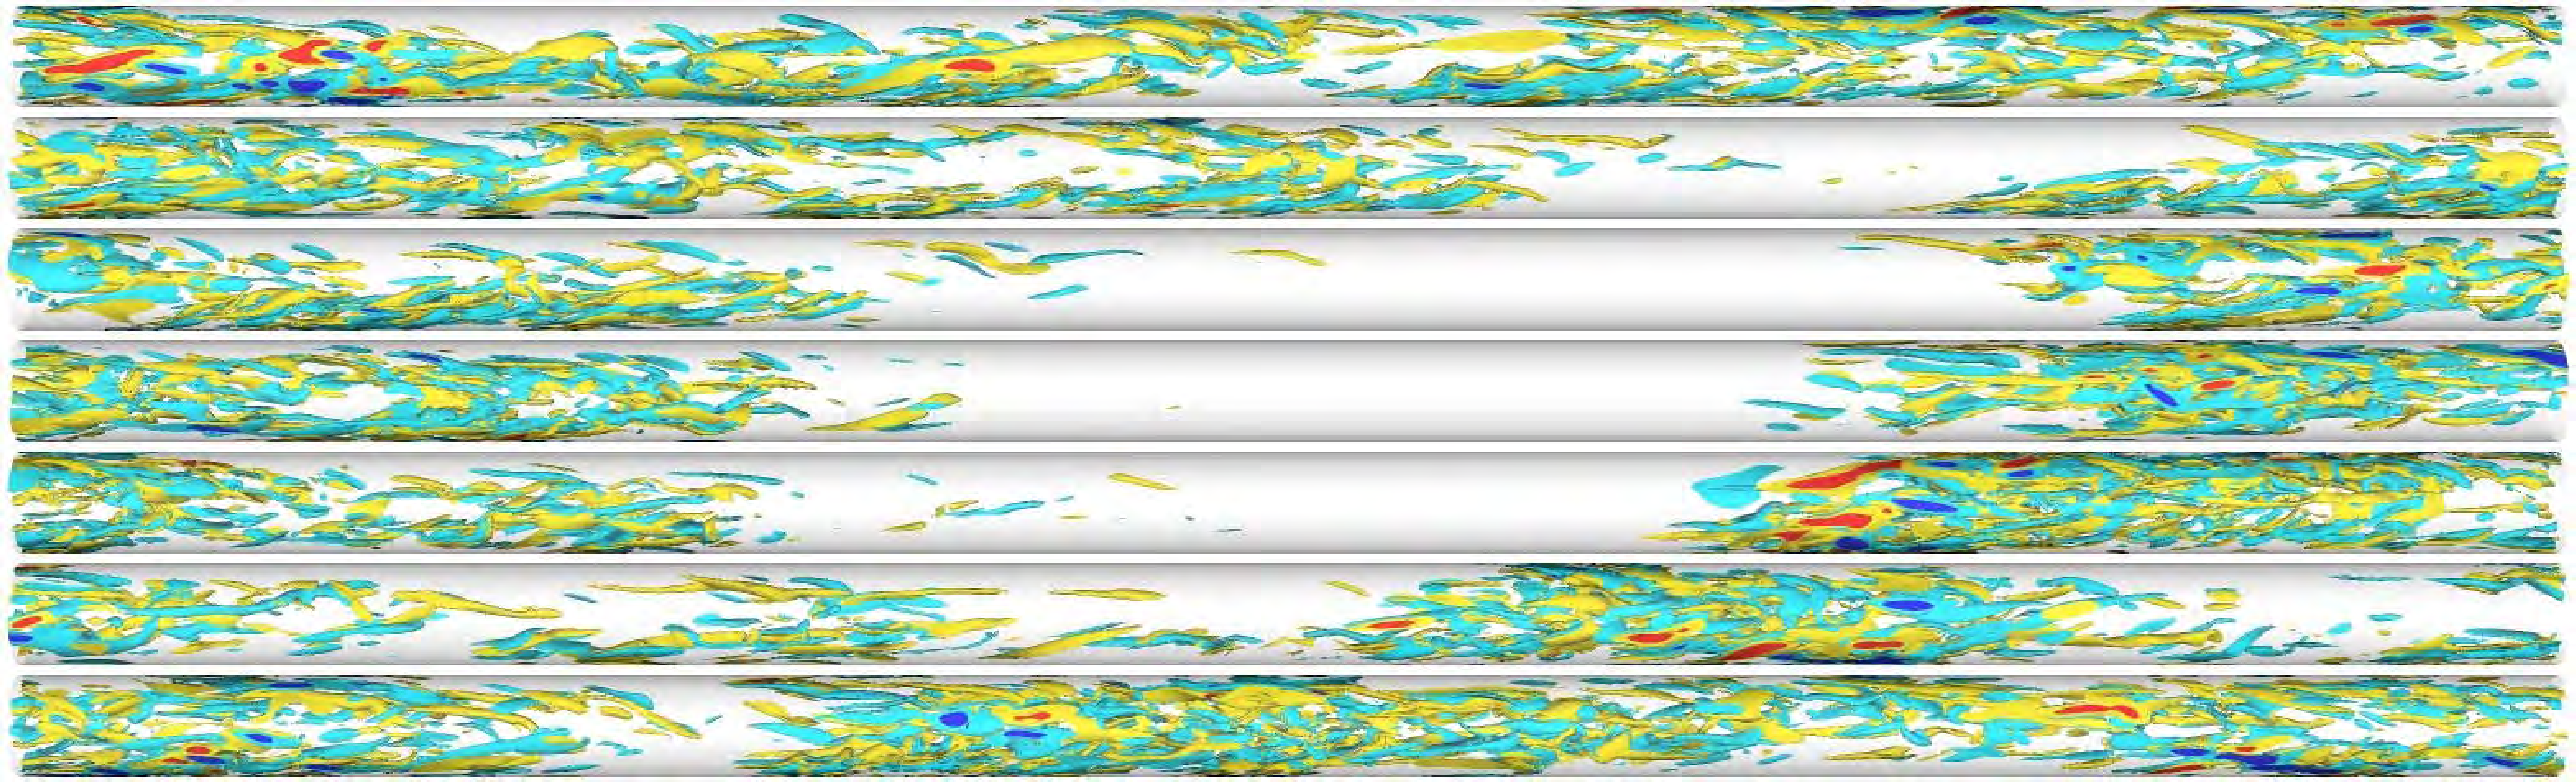
\includegraphics[width=1.0\textwidth]{AviHof13fig4}
\end{center}
pipe flow close to onset of turbulence
\footnote{M.~Avila and B.~Hof, {Phys. Rev. \bf E 87} (2013)}

\bigskip

but we have \textcolor{red}{\Huge hit a wall} :

\hfill exact coherent structures are too unstable to compute
\end{frame}

\begin{frame}{another example of large space-time domain simulation}
\begin{block}{complex Ginzburg-Landau}
  \includegraphics[width=0.515\textwidth] %,height=0.5\textheight,clip=true]
  {cGLdefturbabs}
  \hfill
  (will return to this)
\end{block}

{\footnotesize
[horizontal] space $\ssp \in [-L/2,L/2]$
\qquad
{[up]} time evolution
}

\hfill {\scriptsize \color{orange} codeinthehole.com/static/tutorial/coherent.html}
\end{frame}

\begin{frame}{(1+1) space-time dimensional ``Navier-Stokes''}
% conceptually not ready yet to explore \\ %the inertial manifold of
% $(1+3)$\dmn\ turbulence - start instead with

% \bigskip

\begin{block}{\KS\ $(1+1)$\dmn\ PDE}
\[
  u_t + u \triangledown u \,=\,
    {\color{red}-}\triangledown^2 u {\color{red}-\triangledown^4 u}
    \,,\qquad   x \in [-L/2,L/2]
    \,,
\]
\end{block}

\bigskip

describes spatially extended systems such as
\begin{itemize}
 \item flame fronts in combustion
 \item reaction-diffusion systems
 \item \ldots
\end{itemize}
\end{frame}

\begin{frame}{another example : \KS\ on a large domain}
\begin{center}
  \includegraphics[width=0.6\textwidth] %,height=0.5\textheight,clip=true]
  {ks_largeL_cbar_200} %{ksevol-fig} %{ks_largeL_cbar}
\end{center}

{\footnotesize
[horizontal] space $\ssp \in [0,L]$
\qquad
{[up]} time evolution
}

\begin{itemize}
\item turbulent behavior
\item simpler physical, mathematical and computational setting than Navier-Stokes
\end{itemize}
\end{frame}

\begin{frame}{compact space, infinite time cylinder}
\begin{center}
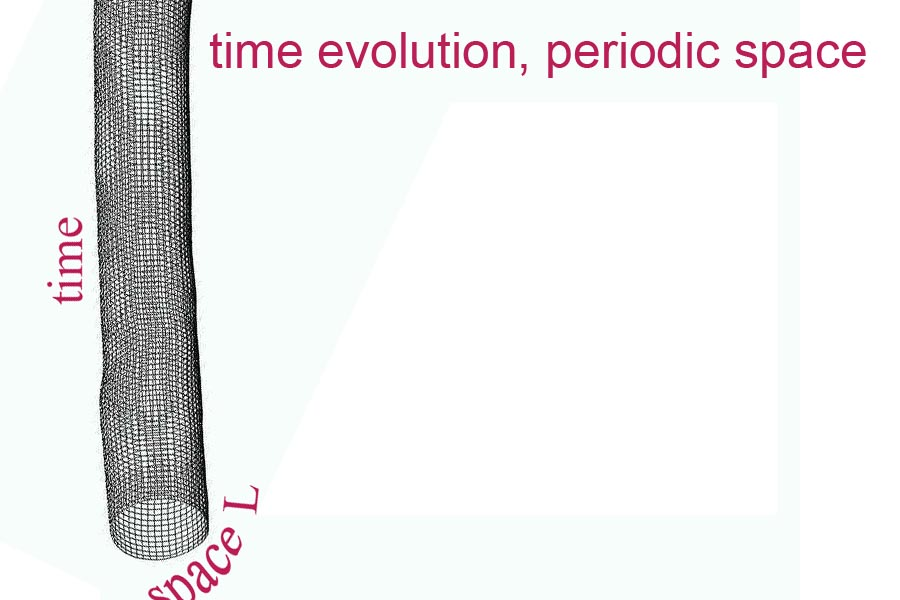
\includegraphics[width=0.9\textwidth]{cylinderTime}
\end{center}
% \hfill \color{red}{(impossible without xxx)}
so far : Navier-Stokes on compact spatial domains, all times
\end{frame}

\begin{frame}{compact space, infinite time} % \KS}
\begin{block}{\KS\ equation}
\[
  u_t \,=\,
    -({\color{red}+}\triangledown^2 +{\color{red}\triangledown^4}) u
    - u \triangledown u
    \,,\qquad   x \in [-L/2,L/2]
    \,,
\]
\end{block}

\bigskip

\begin{block}{in terms of discrete spatial Fourier modes}
$N$ ordinary differential equations (ODEs) in time
\[
\dot{\Fu}_k(\zeit) = ( q_k^2 - q_k^4 )\, \Fu_k(\zeit)
- i \frac{q_k}{2} \!\sum_{k'=0}^{N-1} \!\!\Fu_{k'}(\zeit) \Fu_{k-k'}(\zeit)
\,.
%\label{e-Fks}
\]
\end{block}
\end{frame}


\subsection{types of solutions}
\begin{frame}{evolution of \KS\ on small $L=22$ cell}
\begin{center}
  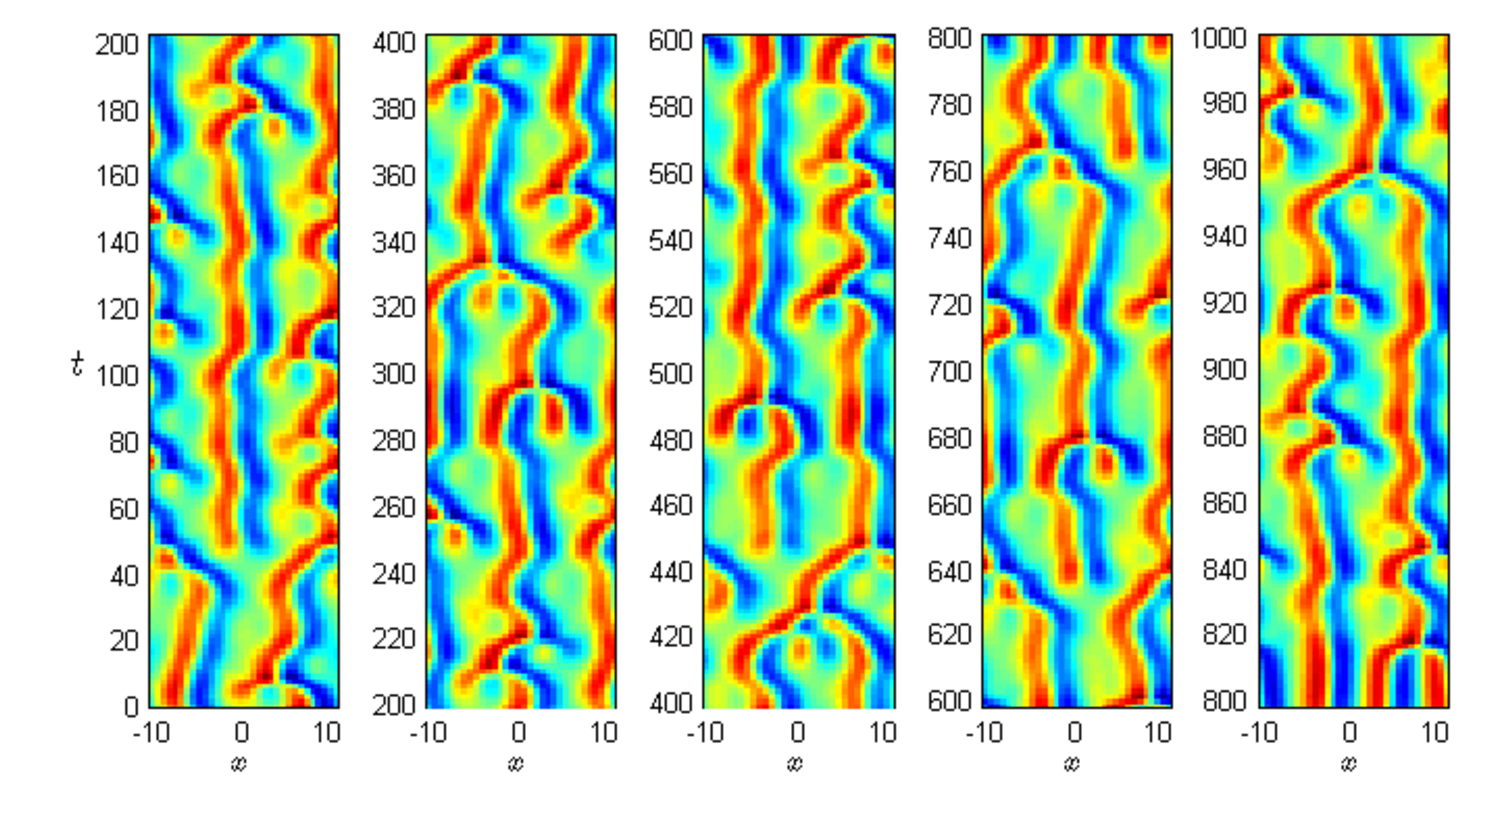
\includegraphics[width=0.9\textwidth,clip=true]{ks_L22_long_orbit}
\end{center}
horizontal: $x \in [-11,11]$
\\
vertical: time
\\
color: magnitude of $u(x,t)$
\end{frame}

\begin{frame}{part 2}
\begin{enumerate}
              \item
    \textcolor{gray}{\small
turbulence in large domains
        }
              \item
    {\Large
space is time
    }\textcolor{gray}{\small
              \item
spacetime
              \item
bye bye, dynamics
                    }
            \end{enumerate}
\end{frame}

\begin{frame}{yes, but}
\begin{center}
{\huge is space time?}
\end{center}
\end{frame}

\begin{frame}{can do : compact time, infinite space cylinder}
\begin{center}
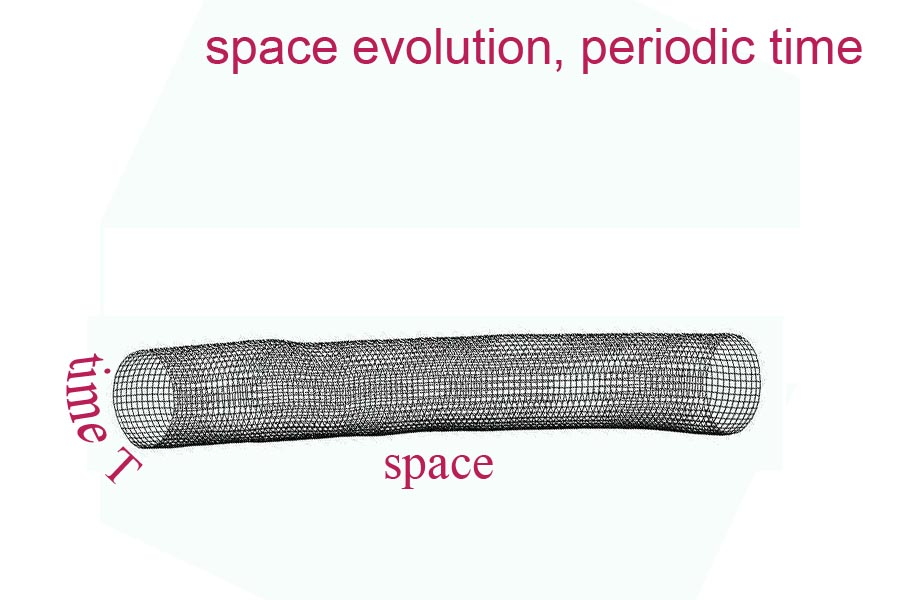
\includegraphics[width=0.9\textwidth]{cylinderSpace}
\end{center}
% \hfill \color{red}{(impossible without xxx)}
\end{frame}

\begin{frame}{compact time, infinite space}
\begin{block}{ \KS\ as four fields \\ 1st order in spatial derivatives}
\bea
    u_\zeit &=&  - u u_\conf
    -u_{\conf \conf}-u_{\conf \conf \conf \conf}\,,
    % \label{e-ks}
\continue
    u^{(0)} &\equiv& u \, , \quad
    u^{(1)} \equiv u_{\conf} \, , \quad
    u^{(2)} \equiv u_{\conf \conf} \, , \quad
    u^{(3)} \equiv u_{\conf \conf \conf}
                        \nonumber
\eea
\end{block}

\begin{block}{evolve four 1st order PDEs $u^{(j)}(\zeit, \conf)$ in $\conf$,}
periodic boundary condition in time
              $u(\conf, \zeit) = u(\conf, \zeit + \period{})$
\bea
    u^{(0)}_{\conf} &=& u^{(1)} \,,\quad
    u^{(1)}_{\conf}  =  u^{(2)} \,,\quad
    u^{(2)}_{\conf}  =  u^{(3)} \continue
    u^{(3)}_{\conf} &=& - u^{(0)}_{\zeit} - u^{(2)} - u^{(0)} u^{(1)}
                        \nonumber
\eea
\end{block}

\bigskip

initial
$u^{(0)}(\conf_0, \zeit)$,
$u^{(1)}( \conf_0, \zeit)$,
$u^{(2)}( \conf_0, \zeit)$,
$u^{(3)}( \conf_0, \zeit)$
    \\
specified for  $\zeit \in [0, \period{})$, at a fixed space point $\conf_0$
\end{frame}

\begin{frame}{a time-invariant \eqv, spatial \po}
\begin{center}
  \begin{minipage}[height=.45\textheight]{.45\textwidth}
    \centering \small{\texttt{(a)}}
    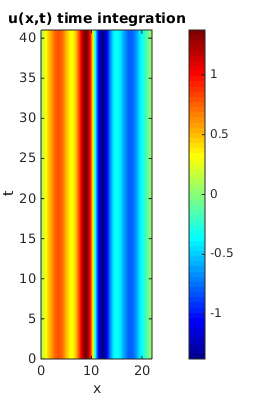
\includegraphics[width=\textwidth,height=.45\textheight]{MNGeq1time}
  \end{minipage}
  \begin{minipage}[height=.45\textheight]{.45\textwidth}
    \centering \small{\texttt{(b)}}
    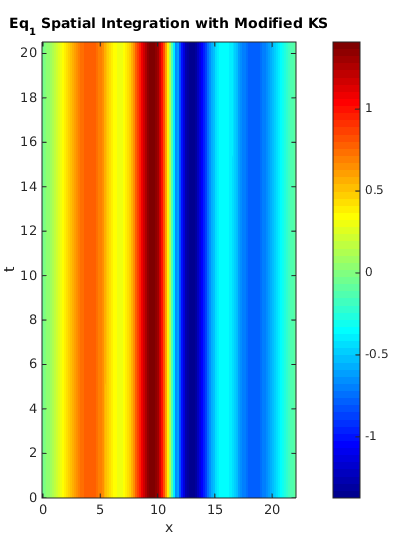
\includegraphics[width=\textwidth,height=.45\textheight]{MNGeq1space}
  \end{minipage}
\end{center}
   %\caption{
  evolution of $\EQV{1}$ : (a) in time, (b) in space
   \\
   initial condition for the spatial integration is the time strip
   $u(\conf_0,\zeit)$, $\zeit = [0,\period{})$, where time period
   $\period{} =0$, spatial $x$ period is $L=22$.
   % }\label{fig:MNGeqva1spttmp}

\vfill\hfill        Michelson 1986, Gudorf 2016
\end{frame}

\begin{frame}{part 3}
\begin{enumerate}
              \item
    \textcolor{gray}{\small
turbulence in large domains
              \item
space is time
    }
              \item {\Large
spacetime
    }\textcolor{gray}{\small
              \item
bye bye, dynamics
                    }
            \end{enumerate}
\end{frame}

\begin{frame}{space-time complex Ginzburg-Landau on a large domain}
\begin{block}{goal : enumerate nearly recurrent chronotopes}
  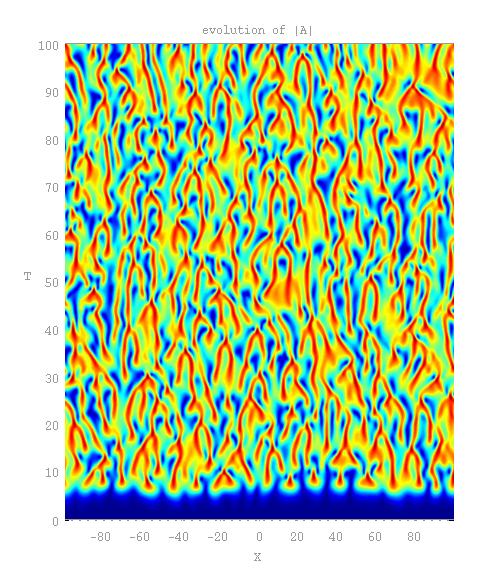
\includegraphics[width=0.4635\textwidth]{cGLdefturbabs}%
~~\raisebox{+3.33ex}[5.5ex][4.5ex]
		 {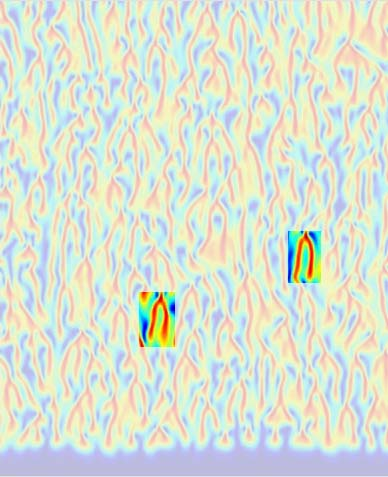
\includegraphics[width=0.36\textwidth]{cGLdefturbclip}}
\end{block}

{\footnotesize
[left-right] space $\ssp \in [-L/2,L/2]$
\qquad
{[up]} time $t\in [0,\period{}]$
}
\end{frame}

\begin{frame}{chronotope
    \footfullcite{LePoTo96}%$^,$\footfullcite{WK09}
}
\begin{bartlett}{
In literary theory and philosophy of language, the chronotope is how
configurations of time and space are represented in language and
discourse.
                }\bauthor{
\HREF{https://en.wikipedia.org/wiki/Chronotope}
{Wikipedia : Chronotope}
                }
\end{bartlett}

\bigskip
\bigskip
%goes without saying : was done by a Soviet scientist first

\begin{itemize}
  \item Mikhail Mikhailovich Bakhtin (1937)
%  \item Politi, Giacomelli, Lepri, Torcini (1996)
%  \item Gutkin and Osipov (2016)
\end{itemize}
\end{frame}

\begin{frame}{use spatiotemporally compact solutions as chronotopes}
\begin{center}
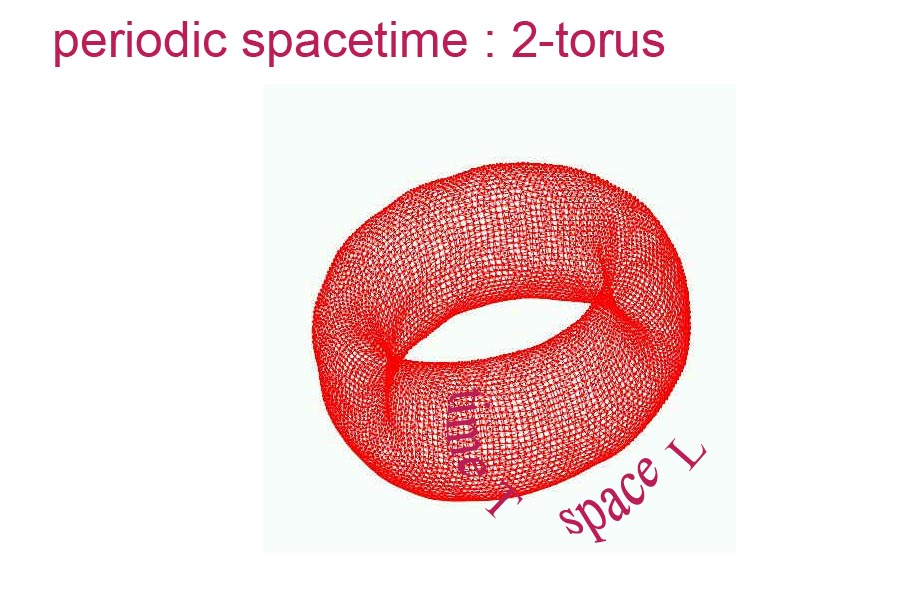
\includegraphics[width=0.9\textwidth]{torusSpTime}
\end{center}
\textcolor{red}{shadows} a small patch of spacetime
% \hfill \color{red}{(impossible without xxx)}
\end{frame}

\begin{frame}{\po s generalize to $d$-tori}

\begin{block}{1 time, 0 space dimensions}
a {\statesp} point is {\em periodic} if its orbit returns to it
after a finite time \period{}; such orbit tiles the time axis
by infinitely many repeats
\end{block}

\bigskip

\begin{block}{1 time, $d$-1 space dimensions}
 a {\statesp} point is {\em spatiotemporally periodic} if
it belongs to \\ an invariant $d$-torus ${\R}$,\\
\ie, a \brick\ $\Mm_{\R}$ that
tiles the lattice state  $\Mm$, \\
with period $\ell_j$ in $j$th lattice direction
\end{block}
\end{frame}

\begin{frame}{a spacetime \twot\ integrated in either time or space}
\begin{center}
  \begin{minipage}[height=.40\textheight]{.35\textwidth}
    \centering \small{\texttt{(a)}}
    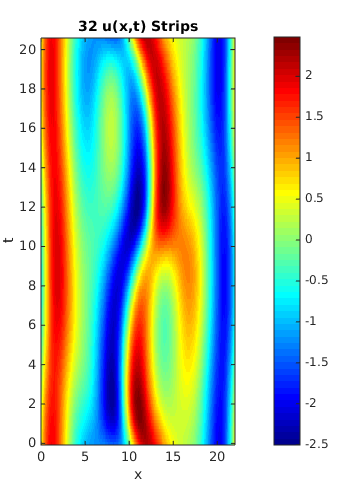
\includegraphics[width=\textwidth,height=.60\textheight]{MNGcomp32xint22}
  \end{minipage}
~~~~~~~~~
  \begin{minipage}[height=.40\textheight]{.35\textwidth}
    \centering \small{\texttt{(b)}}
    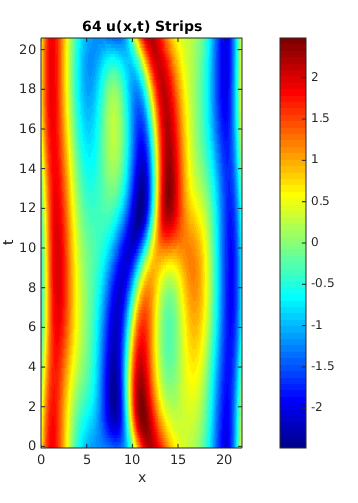
\includegraphics[width=\textwidth,height=.60\textheight]{MNGcomp64xint22}
  \end{minipage}
\end{center}
    (a) old : time evolution. (b) new : space evolution
    \\
    $x=[0,L]$ %22]$,
       initial condition : time periodic line $t = [0,T]$
  %2\,T_{\PPO{10.2}})$
  %\label{fig:MNGcompxint2}

\vfill\hfill        Gudorf 2016
\end{frame}

\begin{frame}{but integrations are uncontrollably unstable}
\begin{center}
{\huge neither} time {\huge nor} space integration {\huge works} \\
for large domains
\end{center}

\vfill
\color{red}{rethink the calculation}
\end{frame}


\begin{frame}{every compact solution is a fixed point on a discrete lattice}
discretize $u_{nm} = u(\conf_n,\zeit_m)$ over
$N M$ points of spatiotemporal periodic lattice $\conf_n = n L/N$,
 $\zeit_m = m \period{}/M$, Fourier transform :
%\beq
%    \Fu_{k,m}^{(i)} = \frac{1}{M} \sum_{\ell = 0}^{M-1}
%    \Fu^{(i)}_{k,\ell} e^{i \omega_\ell \zeit_m}
%    \, , \quad
%    \Fu^{(i)}_{k,\ell} = \sum_{m=0}^{M-1}\Fu_{k,m}^{(i)}  e^{-i \omega_\ell \zeit_m}
%    \, , \quad
%    \mbox{where }
%    \omega_\ell = 2 \pi \ell / \period{} \, .
%\eeq
%
\[
\Fu_{k\ell} \,=\,
  \frac{1}{NM} \sum^{N-1}_{n=0} \sum^{M-1}_{m=0}
  u_{nm} \, e^{-i(q_k\conf_n + \omega_\ell \zeit_m)}
    \,,\quad
q_k = \frac{2 \pi k}{L}
    \,,\;
\omega_\ell = \frac{2 \pi \ell}{\period{}}
% \label{spattempFT}
\]
\KS\ is no more a PDE / ODE, \\
but an algebraic $[N\!\times\!M]$\dmn\ fixed point problem \\
of determining a solution to
\[
\left[- i \omega_\ell - ( q_k^2 - q_k^4 ) \right]\Fu_{k\ell}
+ i \frac{q_k}{2} \!\sum_{k'=0}^{N-1} \sum^{M-1}_{m'=0}\!\!
\Fu_{k'm'} \Fu_{k-k',m-m'}
    =
0
%\,.
%\label{e-FksSpattemp}
\]
\end{frame}

\begin{frame}{every calculation is a spatiotemporal lattice calculation}
field is discretized as
$\Fu_{k\ell}$ values  \\ over
$N M$ points of a periodic lattice

%\medskip

\begin{center}
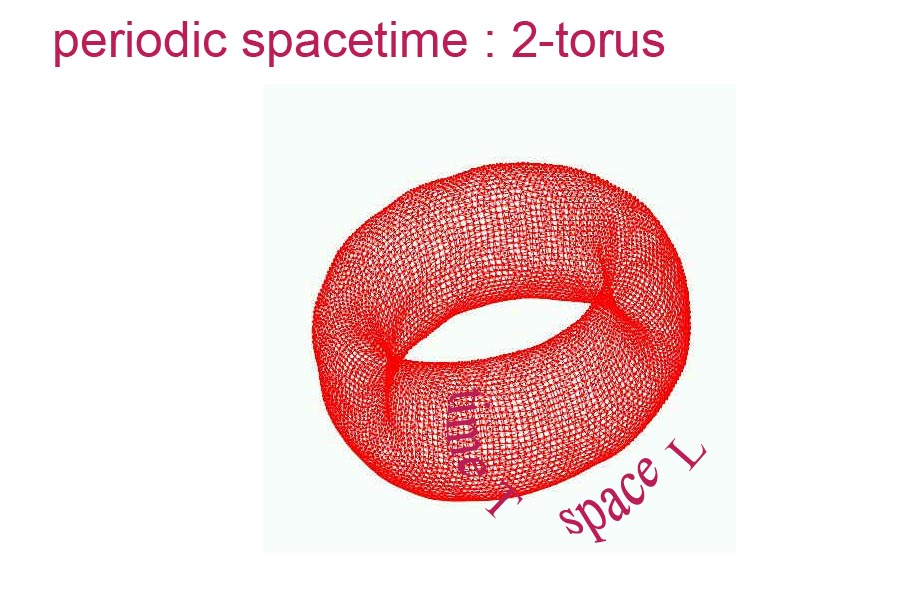
\includegraphics[width=0.9\textwidth]{torusSpTime}
\end{center}
% \hfill \color{red}{(impossible without xxx)}
\end{frame}


\begin{frame}{there is no more time evolution}
solution to \KS\ is now given as
\begin{block}{condition that}
at each lattice point $k\ell$ \\
the tangent field at $\Fu_{k\ell}$
\end{block}
satisfies the equations of motion
\[
\left[- i \omega_\ell - ( q_k^2 - q_k^4 ) \right]\Fu_{k\ell}
+ i \frac{q_k}{2} \!\sum_{k'=0}^{N-1} \sum^{M-1}_{m'=0}\!\!
\Fu_{k'm'} \Fu_{k-k',m-m'}
    =
0
%\,.
%\label{e-FksSpattemp}
\]

\bigskip

this is a \textcolor{red}{local} tangent field constraint on a \textcolor{red}{global} solution

\bigskip

robust : no exponential instabilities as there are no finite time / space integrations

\end{frame}

\begin{frame}{part 4}
\begin{enumerate}
              \item
    \textcolor{gray}{\small
turbulence in large domains
              \item
space is time
              \item
spacetime    }
              \item {\Large
spacetime computations
    }\textcolor{gray}{\small
              \item
bye bye, dynamics
                    }
            \end{enumerate}
\end{frame}


\begin{frame}{how to find solutions ? an ODE example}
\begin{center}
the law of motion : $\qquad \dot{\ssp} = \pVeloc(\ssp)$
\begin{minipage}[c]{0.55\textwidth}
\textcolor{red}{guess loop tangent}
$\lVeloc(\lSpace)
	\neq
\pVeloc(\lSpace)$

	\vskip 0.5cm

\textcolor{green}{periodic orbit}
$\lVeloc(\lSpace)$,~$\pVeloc(\lSpace)$
aligned
\end{minipage}%
~~~~~~~\begin{minipage}[c]{0.40\textwidth}
	\begin{center}
	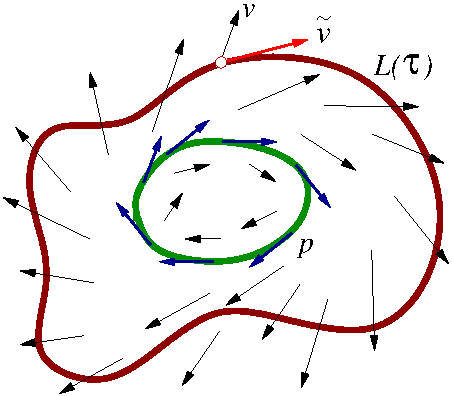
\includegraphics[width=0.7\textwidth]{velocField}
	\end{center}
\end{minipage}
\end{center}
\begin{block}{cost function}%
\[
\costF[\lSpace] =
            \oint_\Loop ds\,(\lVeloc-\pVeloc)^2
    \,;\quad
    \lVeloc = \lVeloc(\lSpace(s,\tau))\,,\,\,
    \pVeloc = \pVeloc(\lSpace(s,\tau))
\,,
% \label{loopCostFct}
\]
\end{block}
\bigskip

penalize\footfullcite{lanVar1}%{ Lan and Cvitanovi\'c, Phys. Rev. (2004)}
 misorientation of the loop tangent
$\lVeloc(\lSpace)$
relative to the true dynamical flow tangent field $\pVeloc(\lSpace)$
\end{frame}

\begin{frame}{how do clouds solve PDEs?}
clouds do not \textcolor{red}{\Huge NOT} {integrate} Navier-Stokes equations

\bigskip\bigskip

\begin{center}
\begin{minipage}[t]{\textwidth}
	\begin{center}
\centerline{
\raisebox{-4.0ex}[5.5ex][4.5ex]
		 {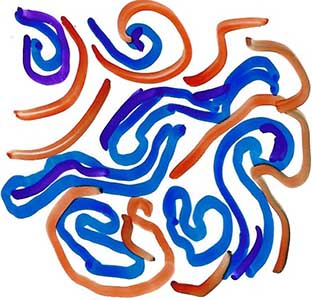
\includegraphics[height=12ex]{Hopf-a}}
~~~ $\Longrightarrow$ ~~ {other swirls} ~~ $\Longrightarrow$ ~~~
	\raisebox{-4.0ex}[5.5ex][4.5ex]
		 {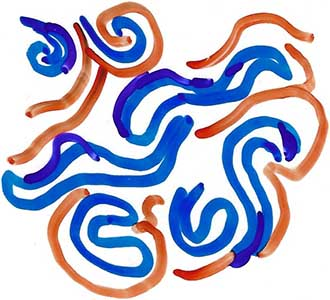
\includegraphics[height=12ex]{Hopf-b}}
          }
	\end{center}
\end{minipage}
\end{center}

do clouds satisfy Navier-Stokes equations?

\bigskip

{\Large yes!}

\centerline{
\textcolor{blue}{they satisfy them \textcolor{red}{\large locally}, everywhere and at all times}
}
\end{frame}

\begin{frame}{the equations imposed as local constraints}
\begin{block}{\KSe}
\[
F(u) = u_t + u_{\conf \conf} + u_{\conf \conf \conf \conf} + u u_{\conf} = 0
\]
\end{block}
\bigskip\bigskip
for example, minimize
\begin{block}{cost function}
\[
G \equiv \frac{1}{2} |F(u,T,L)|^2
%\ee{costfunctional}
\]
\end{block}
\vfill\hfill\textcolor{red}{\Huge need your help !}
\end{frame}

\begin{frame}{Initial guess generation ?}
 \textcolor{blue}{the time scale} : the shortest
`turnover' scale characterized by the period of the shortest \po? Or perhaps
the Lyapunov time?

\bigskip

\textcolor{blue}{the spatial scale} :
$\bar{L}=2\pi\sqrt{2}$, the  most unstable spatial wavelength of the \KS

\bigskip

%%%%%%%%%%%%%%%%%%%%%%%%%%%%%%%%%%%%%%%%%%%%%%%%%%%%%%%%%%%%%%%%
%\label{fig:MNG_spacetime_smoothed} from siminos/spatiotemp/blogMNG.tex
\begin{minipage}[height=.32\textheight]{.30\textwidth}
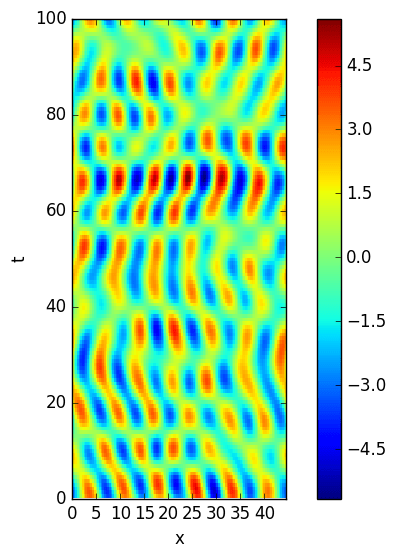
\includegraphics[width=\textwidth,height=.32\textheight]{MNG_T100L44_init}
\end{minipage}

\medskip
initial : spatial $\bar{L}$-modulated random guess
%%%%%%%%%%%%%%%%%%%%%%%%%%%%%%%%%%%%%%%%%%%%%%%%%%%%%%%%%%%%%%%%

\vfill\hfill        Gudorf 2018
\end{frame}

\begin{frame}{Adjoint descent}

\vfill\hfill
M. Farazmand\footfullcite{Faraz15}
\end{frame}

\begin{frame}{KS \twots\ can be found variationally}
%%%%%%%%%%%%%%%%%%%%%%%%%%%%%%%%%%%%%%%%%%%%%%%%%%%%%%%%%%%%%%%%
%\label{fig:MNG_spacetime_smoothed} from siminos/spatiotemp/blogMNG.tex
\begin{minipage}[height=.32\textheight]{.30\textwidth}
\centering \small{\texttt{(a)}}
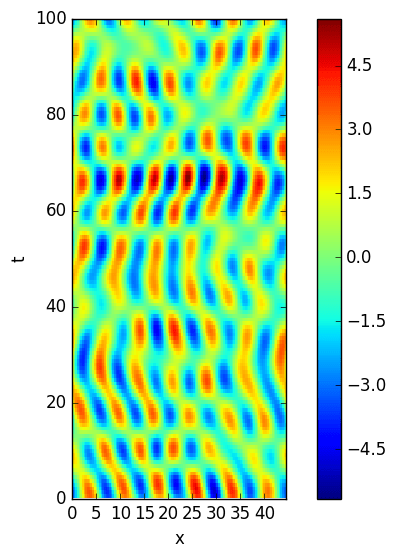
\includegraphics[width=\textwidth,height=.32\textheight]{MNG_T100L44_init}
\end{minipage}
\begin{minipage}[height=.32\textheight]{.30\textwidth}
\centering \small{\texttt{(b)}}
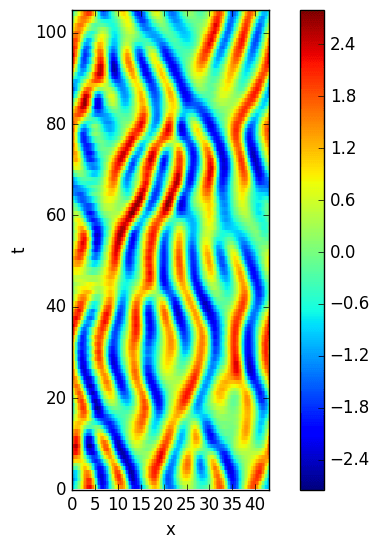
\includegraphics[width=\textwidth,height=.31\textheight]{MNG_T100L44_final}
\end{minipage}

\medskip
(a) initial : $\bar{L}=2\pi\sqrt{2}$ spatially modulated ``noisy'' guess

(b) result : spatiotemporal field \\
 spatial and time periods
 $L=24.07$, $T=31.86$
%%%%%%%%%%%%%%%%%%%%%%%%%%%%%%%%%%%%%%%%%%%%%%%%%%%%%%%%%%%%%%%%

\vfill\hfill        Gudorf 2018
\end{frame}

\begin{frame}{Matrix-free adjoint descent}
\end{frame}

\begin{frame}{Newton descent}
\footfullcite{lanVar1}
\end{frame}

\begin{frame}{Discrete {Lagrangian} methods}
action
\(
S(q)=\int_0^T \!dt\, L(q,\dot{q})
\)
~~+~~
Hamilton’s principle
\(
\delta S(q)=0
\)
\[
\mbox{discretize  }
\int_{t_k}^{t_{k+1}} L(q,\dot{q})\,dt
    \approx
{\Delta t} L(q_k,q_{k+1})
\,.
\]
symplectic methods preserve phase-space areas\footfullcite{MarWes01}

    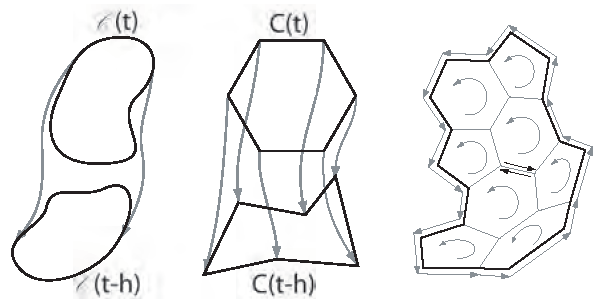
\includegraphics[width=.45\textwidth]{GDPSS06fig5}
%\caption{\label{fig:GDPSS06fig5}

(left) Kelvin's circulation
advected by the flow is constant

(middle) the discrete version, on a Voronoi loop

(right) circulation is constant on any discrete loop.
\end{frame}

\begin{frame}{Discrete {Lagrangian} codes ?}
so far, no codes for \\
discretized spatiotemporal action / Lagrangian density
\[
S =\int\!dq^d\, {\cal L}(q)
\]
symplectic Euler incompressible fluid dynamics
time-evolution codes exist\footfullcite{PMTKMD11}

claim : can apply to  non-conservative system
\vfill\hfill \textcolor{red}{\NS ?}
\end{frame}

%%%%%%%%%%%%%%%%%%%%%%%%%%%%%%%%%%%%%%%%%%%%%%%%%%%%%%%%%%%%%%%%
\begin{frame}{part 5}
\begin{enumerate}
              \item
    \textcolor{gray}{\small
turbulence in large domains
              \item
space is time
    }
              \item
    {\Large
bye bye, dynamics
    }
            \end{enumerate}
\end{frame}

\begin{frame}{in future there will be no future}
\begin{center}
{\huge goodbye}
\end{center}

\vfill

to long time and/or space integrators

\medskip

\hfill they never worked and could never work
\end{frame}

\begin{frame}{life outside of time}
\textcolor{red}{the trouble}:

forward time-integration codes too unstable

\bigskip
\bigskip

\textcolor{blue}{multishooting inspiration}:
 replace a guess that a  \textcolor{blue}{point} is on the periodic
orbit by a guess of the \textcolor{blue}{entire orbit}.

\bigskip

$\to$

\bigskip

spatio-temporally periodic solutions of classical field theories
can be found by \textcolor{blue}{variational methods}
\end{frame}

\begin{frame}{can computers}

\vfill

{\Huge
do this ?
                  }

\vfill

\end{frame}


\begin{frame}{the answer is}

\vfill

{\Huge
scalability
                  }

\vfill

%\hfill in the spirit of this workshop
\end{frame}

\begin{frame}{compute locally, adjust globally}
\begin{block}{computing literature}
parallelizing {\color{red}spatiotemporal}
computation is FLOPs intensive, but more robust than
integration forward in time
\end{block}

\vfill\hfill
it's rocket science\footfullcite{WGBGQ13}
%\footnote{{\tiny Q. Wang \etal,}\HREF{https://doi.org/10.1063/1.4819390}
%{\tiny\em Towards scalable parallel-in-time turbulent flow simulations},
%{\tiny Physics of Fluids (2013)}}
\end{frame}

\begin{frame}{
towards scalable parallel-in-time turbulent flow simulations
}
\begin{block}{future :}%
processor speed $\to$ limit

\medskip

number of cores $\to 10^6 \to \cdots$

\medskip
\end{block}

\emph{Wang et al (2013)
    \footfullcite{WGBGQ13}%$^,$\footfullcite{Ihara66}
    :} % Gomez, Blonigan, Gregory and Qian 2013 :}

next-generation simulation paradigm : space-time parallel
simulations, on discretized $4D$ space-time
computational domains, with each computing core handling a space-time lattice cell

\bigskip

compared to time-evolution solvers:
significantly higher level of concurrency, reduction the ratio of
inter-core communication to floating point operations

\bigskip

$\qquad\qquad\Rightarrow$ a path towards exascale DNS of turbulent flows
\end{frame}

\begin{frame}{KS \twots\ found by rocket science}
\footfullcite{WGBGQ13}

%%%%%%%%%%%%%%%%%%%%%%%%%%%%%%%%%%%%%%%%%%%%%%%%%%%%%%%%%%%%%%%%
% FIG. 18. of {WGBGQ13}
\begin{minipage}[height=.52\textheight]{.30\textwidth}
\centering
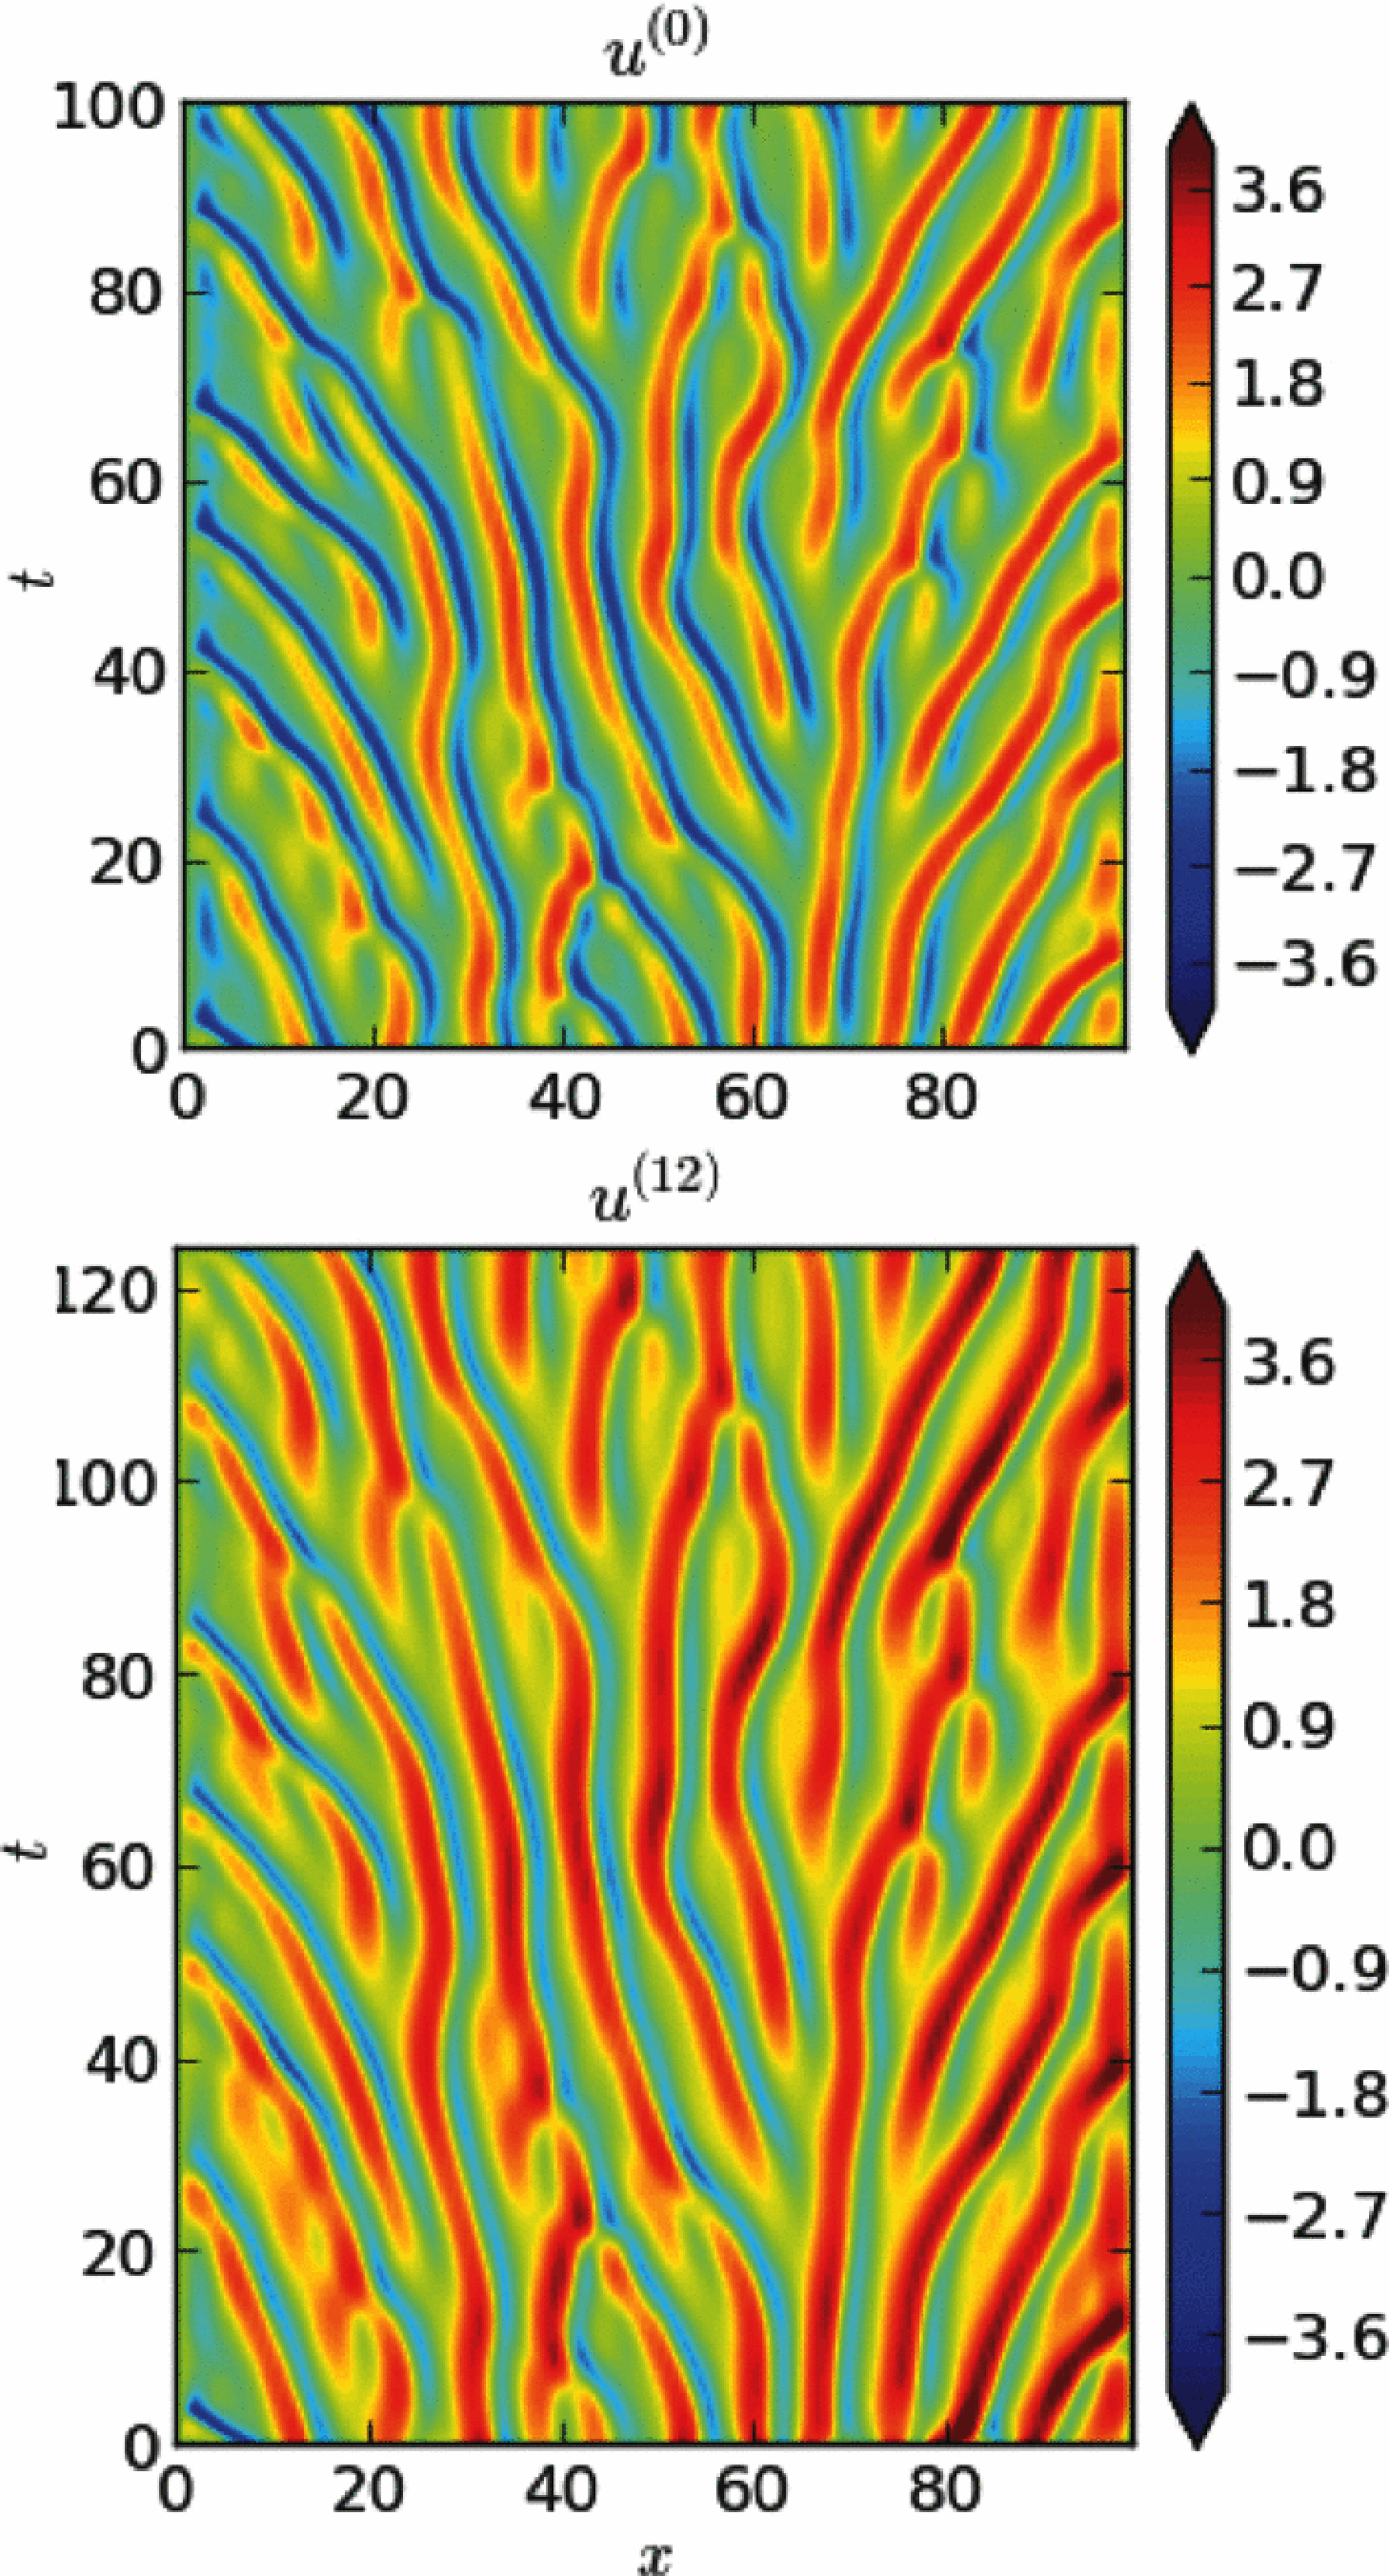
\includegraphics[width=\textwidth,height=.70\textheight]{WGBGQ13fig18}
\end{minipage}
\begin{minipage}[height=.52\textheight]{.60\textwidth}
the initial guess

\bigskip

 the converged solution  $u(x,t)$
\end{minipage}
\end{frame}


\begin{frame}{clouds do not solve PDEs}

%and do they care what PST hour is it?
%\\
%and at what longitude are they?
%\\
do clouds integrate Navier-Stokes equations?

\begin{center}
\centerline{\textcolor{red}{\Huge NO!}}
%\end{center}
%for weather prediction, we store sets of weather sequences
%\bigskip\bigskip

%\begin{center}
\begin{minipage}[t]{\textwidth}
	\begin{center}
%\vspace{2ex}
\centerline{
\raisebox{-4.0ex}[5.5ex][4.5ex]
		 {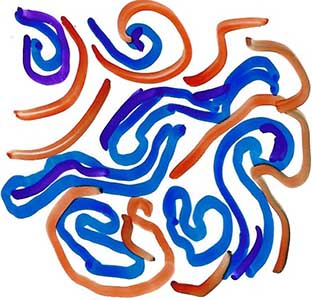
\includegraphics[height=12ex]{Hopf-a}}
~~~ $\Longrightarrow$ ~~ {other swirls} ~~ $\Longrightarrow$ ~~~
	\raisebox{-4.0ex}[5.5ex][4.5ex]
		 {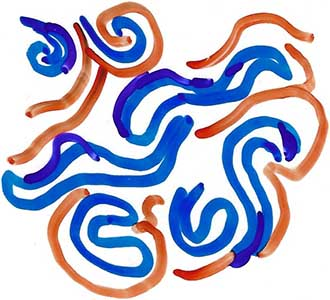
\includegraphics[height=12ex]{Hopf-b}}
          }
	\end{center}
\end{minipage}
\end{center}

at any spacetime point Navier-Stokes equations describe the local tangent space

\bigskip

\centerline{
\textcolor{blue}{they satisfy them \textcolor{red}{\large locally}, everywhere and at all times}
}
\end{frame}


\begin{frame}{summary}
\begin{enumerate}
              \item
study turbulence in infinite spatiatemporal domains
              \item
theory : classify all spatiotemporal tilings
              \item
numerics : future is spatiotemporal
\end{enumerate}

\vfill

there is no more time

\medskip

there is only enumeration of spacetime solutions
\end{frame}

\end{document}
